\documentclass[../Tesi_Jiahao_Miao_986136.tex]{subfiles}

\begin{document}

\section{Inversion of the Laplace transform}

In order to find the quark jet mass distribution $J^q(Q^2,k^2)$ or $R_T(\tau)$, we have to perform the inverse Laplace transform via 
the Mellin's inversion formula (or the Bromwich integral) given by the line integral: 

\begin{equation} \label{eq:inverse_laplace}
    J^q(Q^2,k^2) = \frac{1}{2\pi i} \lim_{T \to \infty}\int_{C-iT}^{C+iT} \dd \nu e^{\nu k^2} \tilde{J}^q_\nu \qty(Q^2),
\end{equation}

where C is a real number such that it is at the right of all singularities of the integrand in the complex plane and
the function $\tilde{J}^q_\nu(Q^2)$ has to be bounded on the line.

Instead of working with the differential quark jet mass distribution $J^q$, it more convenient to deal with
the mass fraction $R^q(w)$, which gives the fraction of jets with masses less than $wQ^2$ (cumulant distribution):

\begin{equation}\label{eq:jet mass fraction}
    R^q(w) = \int_0^\infty J^q(Q^2,k^2)\Theta(wQ^2-k^2) \dd k^2.
\end{equation}

Using the integral representation of the Heaviside step function \cref{eq:heaviside_integral_representation}:

\begin{equation}
    \Theta(wQ^2-k^2) = \frac{1}{2\pi i} \lim_{T \to \infty}\int_{C-iT}^{C+iT} \frac{\dd \nu}{\nu} e^{\nu (wQ^2-k^2)},
\end{equation}

we recognize the Laplace transform of the quark jet mass distribution \cref{eq:laplace_jet_mass}

\begin{align}
    \begin{split}\label{eq:Rw mass fraction}
        R^q(w) &= \frac{1}{2\pi i} \lim_{T \to \infty} \int_{C-iT}^{C+iT} \frac{\dd \nu}{\nu} e^{w \nu Q^2} \int_0^\infty J^q(Q^2,k^2) e^{-\nu k^2} \dd k^2 \\
        &= \frac{1}{2\pi i} \lim_{T \to \infty} \int_{C-iT}^{C+iT} \frac{\dd \nu}{\nu} e^{w \nu Q^2} \tilde{J}^q_\nu(Q^2) \\
        &= \frac{1}{2\pi i} \lim_{T \to \infty} \int_{C-iT}^{C+iT} \frac{\dd \nu}{\nu} e^{w \nu Q^2} e^{\mathcal{F}(\alpha_s,\ln(\nu Q^2))}\\
        &= \frac{1}{2\pi i} \lim_{T \to \infty} \int_{C'-iT}^{C'+iT} \frac{\dd N}{N} e^{w N} e^{\mathcal{F}(\alpha_s,\ln N)},
    \end{split}
\end{align}

where $N=\nu Q^2$ and $\mathcal{F}$ has the logarithms expansion:

\begin{align}
    \begin{split}
    \mathcal{F}(\alpha_s,\ln N) &= f_1(b_0 \alpha_s \ln N) \ln N + f_2(b_0 \alpha_s \ln N) + f_3(b_0 \alpha_s \ln N) \alpha_s \\
    &+ f_4(b_0 \alpha_s \ln N) \alpha_s^2 + f_5(b_0 \alpha_s \ln N) \alpha_s^3 + \order{\alpha_s^4}.
\end{split}
\end{align}

Since the function $\mathcal{F}$ in the exponent varies more slowly with N than $wN$, we can introduce the integration variable $u=wN$
so that $\ln N = \ln u +\ln \frac{1}{w} = \ln u + L$ and Taylor expand with respect to $\ln u$ around $0$, which is equivalent to expanding 
the original function $\mathcal{F}$ w.r.t $\ln N$ around $\ln N \approx \ln \frac{1}{w}\equiv L$:

\begin{align}
    \begin{split}\label{eq:Rw expansion}
       R^q(w) &= \frac{1}{2\pi i} \int_C \frac{\dd u}{u} e^{u} e^{\mathcal{F}(\alpha_s,\ln u + L)} \\
       &\stackrel{\text{Taylor}}{=} \int_C \frac{\dd u}{2\pi i} e^{u-\ln u} e^{\mathcal{F}(\alpha_s,L)+\sum_{n=1}^\infty \frac{\mathcal{F}^{(n)}(\alpha_s,L)}{n!}  \ln^n u}\\
       &= e^{\mathcal{F}(\alpha_s,L)} \int_C \frac{\dd u}{2\pi i} e^{u-\ln u} e^{\sum_{n=1}^\infty \frac{\mathcal{F}^{(n)}(\alpha_s,L)}{n!}  \ln^n u},
    \end{split}
\end{align}

where the integral is intended as before, along the line $C$ to the right of all singularities of the integrand, and 

\begin{equation}
    \mathcal{F}^{(n)}(\alpha_s,L) = \pdv[n]{\mathcal{F}(\alpha_s,\ln u + L )}{(\ln u)} \eval_{\ln u = 0}.
\end{equation}

The $n$-th derivative of $\mathcal{F}$ w.r.t $\ln u$ evaluated at $\ln u = 0$ is 
at most of logarithmic order $\alpha_s^{n+k-1}L^k$ \cite{CATANI19933}, so in order to achieve $\text{N}^4\text{LL}$ accuracy we need to compute the first four derivatives of $\mathcal{F}$ w.r.t $\ln u$ and 
neglect the terms of order $\order{\alpha_s^4}$ that appear in the derivation. We obtain the following expressions: 

\begin{flalign}
    \begin{split} \label{eq:derivative F1}
        \mathcal{F}^{(1)}(\alpha_s,L) &= f_1(\lambda )+\lambda  f_1'(\lambda )+\alpha_s b_0 f_2'(\lambda )+\alpha_s^2 b_0 f_3'(\lambda )+\alpha_s^3 b_0 f_4'(\lambda )\\
        &+ \order{\alpha_s^n L^{n-3}},
    \end{split}
\end{flalign}

\begin{flalign}
    \begin{split}\label{eq:derivative F2}
        \mathcal{F}^{(2)}(\alpha_s,L) &= 2 \alpha_s b_0 f_1'(\lambda ) + \alpha_s b_0 \lambda  f_1''(\lambda )+\alpha_s^2 b_0^2 f_2''(\lambda )+ \alpha_s^3 b_0^2 f_3''(\lambda )\\
        &+ \order{\alpha_s^n L^{n-3}},
    \end{split}
\end{flalign}

\begin{flalign}
    \begin{split}\label{eq:derivative F3}
        \mathcal{F}^{(3)}(\alpha_s,L) &=  3 \alpha_s^2 b_0^2 f_1''(\lambda )+\alpha_s^2 b_0^2 \lambda  f_1^{(3)}(\lambda )+\alpha_s^3 b_0^3 f_2^{(3)}(\lambda )+ \order{\alpha_s^n L^{n-3}},
    \end{split}
\end{flalign}

\begin{flalign}
    \begin{split}\label{eq:derivative F4}
        \mathcal{F}^{(4)}(\alpha_s,L) &= 4 \alpha_s^3 b_0^3 f_1^{(3)}(\lambda ) +\alpha_s^3 b_0^3 \lambda  f_1^{(4)}(\lambda )+ \order{\alpha_s^n L^{n-3}},
    \end{split}
\end{flalign}

Here $\lambda = \alpha_s b_0 L$ and derivative w.r.t $\ln u$ and then evaluated at $\ln u = 0$, or equivalently derivative w.r.t $L$ gives the same result.

After recasting the expansion presented in \cref{eq:Rw expansion} using the expression \\
$\gamma(\alpha_s,L) = f_1(\lambda) + \lambda f_1'(\lambda)$ from \cite{CATANI19933}, 
and defining $\mathcal{F}^{(1)}_{res}(\alpha_s,L) \equiv \mathcal{F}^{(1)}(\alpha_s,L) - \gamma(\alpha_s,L)$, we proceed to expand the second exponential with respect to $\ln u$ around 0, 
following the approach outlined in \cite{Aglietti:2002ew}. This yields the subsequent expansion:

\begin{align}
    \begin{split}
        R^q(w) &= e^{\mathcal{F}(\alpha_s,L)} \int_C \frac{\dd u}{2\pi i} e^{u-(1-\gamma(\alpha_s,L))\ln u} e^{\mathcal{F}^{(1)}_{res}(\alpha_s,L) \ln u +\sum_{n=2}^\infty \frac{\mathcal{F}^{(n)}(\alpha_s,L)}{n!}  \ln^n u}\\
        &= \int_C \frac{\dd u}{2\pi i} e^{u-(1-\gamma(\alpha_s,L))\ln u} \biggl( 1 + \mathcal{F}^{(1)}_{res}\ln u +\frac{1}{2}\qty( \mathcal{F}^{(2)}+(\mathcal{F}^{(1)}_{res})^2)\ln^2 u \\
        &+ \frac{1}{6}\qty(\mathcal{F}^{(3)} + 3 \mathcal{F}^{(2)}\mathcal{F}^{(1)}_{res} + (\mathcal{F}^{(1)}_{res})^3 ) \ln^3 u \\
        &+ \frac{1}{24}\qty(\mathcal{F}^{(4)} + 3(\mathcal{F}^{(2)})^2 + 4 \mathcal{F}^{(3)} \mathcal{F}^{(1)}_{res} + 6 \mathcal{F}^{(2)} (\mathcal{F}^{(1)}_{res})^2 + (\mathcal{F}^{(1)}_{res})^4 )\ln^4 u \\
        &+ \order{\ln^5 u} \biggr).
    \end{split}
\end{align}

Lastly, we utilize the following result to evaluate the integral presented in \cref{eq:jet mass fraction}:

\begin{equation}\label{eq:magic_integral}
    \int_C \frac{\dd u}{2\pi i} \ln^k u e^{u-(1-\gamma(\alpha_s,L))\ln u} = \dv[k]{\gamma} \frac{1}{\Gamma(1-\gamma(\alpha_s,L))},
\end{equation}

where $\Gamma$ is the Euler $\Gamma$-function, notice that for $k=0$ the integral is the Hankel integral representation of the $\Gamma$-function:

\begin{equation}\label{eq:hankel_integral_representation}
    \frac{1}{2\pi i}\int_C \dd u e^{u} u^{-(1-\gamma(\alpha_s,L))} = \frac{1}{\Gamma(1-\gamma(\alpha_s,L))}.
\end{equation}

The reciprocal of the Euler $\Gamma$-function is an entire function, meaning that it has no singularities in the complex plane, it's holomorphic everywhere.
The above integral \cref{eq:magic_integral} can be evaluated by differentiating with respect to $\gamma(\lambda)$ $k$ times, and it is straightforward to see that each derivation inside the integral
gives a factor of $\ln u$. Interchaning the order of derivation and integration is justified by the fact that the integral:
\begin{itemize}
    \item  is a contour integral whose contour doesn't depent on $\gamma(\lambda)$, and the function is holomorphic in the complex plane for each value of $\gamma(\lambda) \in (\infty,0]$ (\cref{fig:gamma_lambda})
    \item  is dominated by the exponential factor $e^{u - (1-\gamma(\lambda)) \ln u}$ as long as $\Re{u}>0$.  
\end{itemize}

\begin{figure}
    \centering
    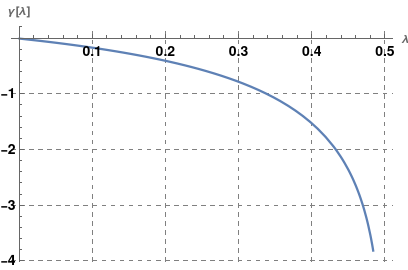
\includegraphics[width=0.5\textwidth]{figures/gamma_lambda.png}
    \caption{Plot of $\gamma(\lambda)$ in the range of interest $0<\lambda<\frac{1}{2}$}
    \label{fig:gamma_lambda}
\end{figure}
 
\begin{align}
    \begin{split}\label{eq:Rw quasi final expansion}
        R^q(w) &= \frac{e^{\mathcal{F}(\alpha_s,L)}}{\Gamma(1-\gamma(\lambda))} \biggl[ 1 + \mathcal{F}^{(1)}_{res} \psi_0 + \frac{1}{2}\qty( \mathcal{F}^{(2)}+(\mathcal{F}^{(1)}_{res})^2) \qty(\psi_0^2-\psi_1) \\
        &+ \frac{1}{6}\qty(\mathcal{F}^{(3)} + 3 \mathcal{F}^{(2)}\mathcal{F}^{(1)}_{res} + (\mathcal{F}^{(1)}_{res})^3 ) \qty(\psi_0^3 -3 \psi_0\psi_1+\psi_2) \\
        &+ \frac{1}{24}\qty(\mathcal{F}^{(4)} + 3(\mathcal{F}^{(2)})^2 + 4 \mathcal{F}^{(3)} \mathcal{F}^{(1)}_{res} + 6 \mathcal{F}^{(2)} (\mathcal{F}^{(1)}_{res})^2 + (\mathcal{F}^{(1)}_{res})^4 ) \\
        &\qty(\psi_0^4 -6 \psi_1 + 3\psi_1^3 +4\psi_0\psi_2 -\psi_3)+ \order{\ln^5 u} \biggr],
    \end{split}
\end{align}

where $\psi_n$ are the polygamma functions all evaluated at $(1-\gamma(\lambda))$, defined as:

\begin{equation}
    \psi_n (z) = \dv[n+1]{z} \ln \Gamma(z) = \dv[n]{z} \frac{\Gamma '(z)}{\Gamma(z)} = \dv[n]{z} \psi_0(z).
\end{equation}

The expression \cref{eq:Rw quasi final expansion} can be verified against Eq.(56) in \cite{Aglietti:2002ew} and Eq.(4.28) in \cite{Monni:2011gb}.
It is noteworthy that they share the same structure within the square brackets, the difference is that they don't include $(\mathcal{F}^{(1)}_{res})^2$ in the second term.
This omission is due to the fact that $(\mathcal{F}^{(1)}_{res})^2$ is a term of order $\order{\alpha_s^2}$ and thus contributes to the N$^3$LL accuracy.

Substituting the expressions \cref{eq:derivative F1,eq:derivative F2,eq:derivative F3,eq:derivative F4} into \cref{eq:Rw quasi final expansion} we obtain:

\begin{flalign}
    R^q(w) &= \frac{e^{\mathcal{F}(\alpha_s,L)}}{\Gamma(1-\gamma)} \biggl[ 1 + \Bigl(\alpha_s^3 b_0 f_4'(\lambda )+\alpha_s^2 b_0 f_3'(\lambda )+\alpha_s b_0 f_2'(\lambda )\Bigr) \psi_0 \\
    &+ \frac{1}{2} \Bigl(\alpha_s^3 \bigl(2 b_0^2 f_2'(\lambda ) f_3'(\lambda )+b_0^2 f_3''(\lambda )\bigr)+ \frac{1}{2} \alpha_s^2 \qty(b_0^2 f_2''(\lambda )+b_0^2 f_2'(\lambda )^2 ) \nonumber\\
    &+\frac{1}{2} \alpha_s \qty(b_0 \lambda  f_1''(\lambda ) + 2 b_0 f_1'(\lambda ) )\Bigr) \qty(\psi_0^2-\psi_1) \nonumber\\
    &+ \frac{1}{6}\Bigl( \alpha_s^3 \bigl(b_0^3 f_2^{(3)}(\lambda )+b_0^3 f_2'(\lambda )^3 + 3 b_0^3 f_2'(\lambda ) f_2''(\lambda )+3 b_0^2 \lambda  f_1''(\lambda ) f_3'(\lambda ) \nonumber\\
    &+6 b_0^2 f_1'(\lambda ) f_3'(\lambda )\bigr) +\frac{1}{6} \alpha_s^2 \bigl(b_0^2 \lambda  f_1^{(3)}(\lambda )+3 b_0^2 \lambda  f_1''(\lambda ) f_2'(\lambda )+3 b_0^2 f_1''(\lambda )\nonumber\\
    &+6 b_0^2 f_1'(\lambda ) f_2'(\lambda )\bigr) \Bigr) \qty(\psi_0^3 -3 \psi_0\psi_1+\psi_2) \nonumber\\
    &+ \frac{1}{24}\Bigl(\alpha_s^3 \bigl(b_0^3 \lambda  f_1^{(4)}(\lambda )+4 b_0^3 \lambda  f_1^{(3)}(\lambda ) f_2'(\lambda )\nonumber\\
    &+4 b_0^3 f_1^{(3)}(\lambda )+6 b_0^3 \lambda  f_1''(\lambda ) f_2''(\lambda )+6 b_0^3 \lambda  f_1''(\lambda ) f_2'(\lambda )^2+12 b_0^3 f_1''(\lambda ) f_2'(\lambda )\nonumber\\
    &+12 b_0^3 f_1'(\lambda ) f_2''(\lambda )+12 b_0^3 f_1'(\lambda ) f_2'(\lambda )^2\bigr)+\frac{1}{8} \alpha_s^2 \bigl(b_0^2 \lambda ^2 f_1''(\lambda )^2+4 b_0^2 f_1'(\lambda )^2\nonumber\\
    &+4 b_0^2 \lambda  f_1'(\lambda ) f_1''(\lambda )\bigr)\Bigr) \qty(\psi_0^4 -6 \psi_1 + 3\psi_1^3 +4\psi_0\psi_2 -\psi_3)+ \order{\ln^5 u} \biggr]\nonumber ,
\end{flalign}

and reorganize as a power series of $\alpha_s$:

\begin{align}\label{eq:Rw final expansion}
        R^q(w) &= \frac{e^{\mathcal{F}(\alpha_s,L)}}{\Gamma(1-\gamma)} \biggl[ 1 + \alpha_s b_0 \Bigl( \psi_0 f_2'(\lambda )  + \frac{1}{2} (\psi_0^2-\psi_1)\bigl( \lambda  f_1''(\lambda ) \\
        &+2  f_1'(\lambda )\bigr)\Bigr) + \alpha_s^2 \Bigl(\frac{1}{8} (\psi_0^4 -6 \psi_1 + 3\psi_1^3 +4\psi_0\psi_2 -\psi_3) \bigl(b_0^2 \lambda ^2 f_1''(\lambda )^2\nonumber\\
        &+4 b_0^2 f_1'(\lambda )^2 +4 b_0^2 \lambda  f_1'(\lambda ) f_1''(\lambda )\bigr)+\frac{1}{6} (\psi_0^3 -3 \psi_0\psi_1+\psi_2) \bigl(b_0^2 \lambda  f_1^{(3)}(\lambda )\nonumber\\
        &+ 3 b_0^2 \lambda  f_1''(\lambda ) f_2'(\lambda )+3 b_0^2 f_1''(\lambda )+6 b_0^2 f_1'(\lambda ) f_2'(\lambda )\bigr)+\frac{1}{2} (\psi_0^2-\psi_1) \nonumber\\
        &\bigl(b_0^2 f_2''(\lambda ) +b_0^2 f_2'(\lambda )^2\bigr) + b_0 \psi_0 f_3'(\lambda )\Bigr) + \alpha_s^3 \Bigl(\frac{1}{24} (\psi_0^4 -6 \psi_1 + 3\psi_1^3 +4\psi_0\psi_2 \nonumber\\
        &-\psi_3) \bigl(b_0^3 \lambda  f_1^{(4)}(\lambda ) +4 b_0^3 \lambda  f_1^{(3)}(\lambda ) f_2'(\lambda ) + 4 b_0^3 f_1^{(3)}(\lambda )+6 b_0^3 \lambda  f_1''(\lambda ) f_2''(\lambda ) \nonumber\\
        &+ 6 b_0^3 \lambda  f_1''(\lambda ) f_2'(\lambda )^2 +12 b_0^3 f_1''(\lambda ) f_2'(\lambda )+12 b_0^3 f_1'(\lambda ) f_2''(\lambda ) + 12 b_0^3 f_1'(\lambda ) f_2'(\lambda )^2\bigr) \nonumber\\
        &+ \frac{1}{2} (\psi_0^2-\psi_1) \bigl(2 b_0^2 f_2'(\lambda ) f_3'(\lambda )+b_0^2 f_3''(\lambda )\bigr) + \frac{1}{6} (\psi_0^3 -3 \psi_0\psi_1\nonumber\\
        &+\psi_2) \bigl(b_0^3 f_2^{(3)}(\lambda )+b_0^3 f_2'(\lambda )^3 +3 b_0^3 f_2'(\lambda ) f_2''(\lambda )+3 b_0^2 \lambda  f_1''(\lambda ) f_3'(\lambda )\nonumber \\
        &+6 b_0^2 f_1'(\lambda ) f_3'(\lambda )\bigr) + b_0 \psi_0 f_4'(\lambda ) \Bigr) + \order{\alpha_s^4} \biggr]\nonumber.
\end{align}

As observed in the previous section, to obtain the Thrust cross section, we simply multiply by 2 all the $f_i$  \cref{eq:f1,eq:f2,eq:f3,eq:f4,eq:f5}. The final resummed expression $R_T(\tau)$ can be written 
as one exponential \cref{eq:resummed_R}, 

\begin{equation}\label{eq:RT_resummed}
    R_T(\tau) = \qty(1 + \sum_{n=1}^{\infty} C_n \bar{\alpha}_s^n)\exp[L g_1(\lambda)  + g_2(\lambda) + g_3(\lambda) \alpha_s + g_4(\lambda) \alpha_s^2 + g_5(\lambda) \alpha_s^3 + \order{\alpha_s^4}].
\end{equation}

To do so, we observe that $\frac{1}{\Gamma(1-\gamma)}= \exp{-\ln(\Gamma(1-\gamma))}$ corrects $f_2$, while the expression in square parenthesis in \cref{eq:Rw final expansion} can be seen 
as the expansion of an exponential for $\alpha_s \to 0$, the reason for this is that since we integrated an exponential function in \cref{eq:Rw mass fraction}, we 
expect to find an exponential function as the result of the integration

\begin{equation}
    \begin{split}\label{eq:expansion exponential}
    \exp(\alpha_s g_3(\lambda) + \alpha_s^2 g_4(\lambda) + \alpha_s^3 g_5(\lambda) + \order{\alpha_s^4}) &= 1+\alpha_s g_3(\lambda)+\frac{1}{2} \alpha_s^2 \qty(g_3^2(\lambda)+2 g_4(\lambda))\\
    &+\frac{1}{6} \alpha_s^3 \qty(g_3^3(\lambda) + 6 g_3(\lambda) g_4(\lambda) + 6 g_5(\lambda))+ \order{\alpha_s^4}.
    \end{split}
\end{equation}

To obtain $g_3(\lambda)$, $g_4(\lambda)$ and $g_5(\lambda)$ we match \cref{eq:Rw final expansion} with \cref{eq:expansion exponential} and obtain the following expressions in which all 
the Polygamma functions $\psi_n$ are evaluated at $1-\gamma(\lambda)$ as before, and the functions $f_i$ are twice the ones obtained in the previous section \cref{eq:f1,eq:f2,eq:f3,eq:f4,eq:f5}: 

\begin{flalign}
    g_1(\lambda) &= f_1(\lambda) \label{eq:g1},\\
    g_2(\lambda) &= f_2(\lambda) -  \ln \Gamma(1- f_1(\lambda)- \lambda f_1'(\lambda)) \label{eq:g2},\\
    g_3(\lambda) &= f_3(\lambda) +   \Bigl( \psi_0(1-\gamma(\lambda)) f_2'(\lambda )  + \frac{1}{2} (\psi_0^2-\psi_1)(1-\gamma)\bigl( \lambda  f_1''(\lambda ) +2  f_1'(\lambda )\bigr)\Bigr) \label{eq:g3},\\
    g_4(\lambda) &=  f_4(\lambda) +  \Bigl(\frac{1}{8} (\psi_0^4 -6 \psi_1 + 3\psi_1^3 +4\psi_0\psi_2 -\psi_3)(1-\gamma(\lambda)) \bigl(b_0^2 \lambda ^2 f_1''(\lambda )^2\label{eq:g4}\\
    &+4 b_0^2 f_1'(\lambda )^2 +4 b_0^2 \lambda  f_1'(\lambda ) f_1''(\lambda )\bigr)+\frac{1}{6} (\psi_0^3 -3 \psi_0\psi_1+\psi_2)(1-\gamma(\lambda)) \bigl(b_0^2 \lambda  f_1^{(3)}(\lambda ) \nonumber\\
    &+ 3 b_0^2 \lambda  f_1''(\lambda ) f_2'(\lambda )+3 b_0^2 f_1''(\lambda )+6 b_0^2 f_1'(\lambda ) f_2'(\lambda )\bigr)+\frac{1}{2} (\psi_0^2-\psi_1)(1-\gamma)\nonumber\\
    &\bigl(b_0^2 f_2''(\lambda )+b_0^2 f_2'(\lambda )^2\bigr) + b_0 \psi_0(1-\gamma(\lambda)) f_3'(\lambda )\Bigr), \nonumber\\
    g_5(\lambda) &=  f_5(\lambda) +  \Bigl(\frac{1}{24} (\psi_0^4 -6 \psi_1 + 3\psi_1^3 +4\psi_0\psi_2 -\psi_3)(1-\gamma(\lambda)) \label{eq:g5}\\
    &\bigl(b_0^3 \lambda  f_1^{(4)}(\lambda ) +4 b_0^3 \lambda  f_1^{(3)}(\lambda ) f_2'(\lambda ) + 4 b_0^3 f_1^{(3)}(\lambda )+6 b_0^3 \lambda  f_1''(\lambda ) f_2''(\lambda ) \nonumber\\
    &+ 6 b_0^3 \lambda  f_1''(\lambda ) f_2'(\lambda )^2 +12 b_0^3 f_1''(\lambda ) f_2'(\lambda )+12 b_0^3 f_1'(\lambda ) f_2''(\lambda ) + 12 b_0^3 f_1'(\lambda ) f_2'(\lambda )^2\bigr) \nonumber\\
    &+ \frac{1}{2} (\psi_0^2-\psi_1)(1-\gamma(\lambda)) \bigl(2 b_0^2 f_2'(\lambda ) f_3'(\lambda )+b_0^2 f_3''(\lambda )\bigr) + \frac{1}{6} (\psi_0^3 -3 \psi_0\psi_1+\psi_2)(1-\gamma) \nonumber\\
    &\bigl(b_0^3 f_2^{(3)}(\lambda )+b_0^3 f_2'(\lambda )^3 +3 b_0^3 f_2'(\lambda ) f_2''(\lambda )+3 b_0^2 \lambda  f_1''(\lambda ) f_3'(\lambda ) +6 b_0^2 f_1'(\lambda ) f_3'(\lambda )\bigr)\nonumber\\
    &+ b_0 \psi_0(1-\gamma) f_4'(\lambda ) \Bigr) . \nonumber
\end{flalign}

The procedure we just described extends the NLL \cite{CATANI19933} and NNLL \cite{Monni:2011gb} results for the analytical Laplace inversion to N$^3$LL and N$^4$LL accuracy.

The thrust differential distribution \cref{eq:differential_cross_section} is obtained by taking the derivative of the thrust cross section 
$R_T(\tau)$ \cref{eq:resummed_R} with respect to $\tau$:

\begin{equation}
    \frac{1}{\sigma} \dv{\sigma}{\tau} = \frac{1}{\tau} \dv{R_T(\tau)}{\ln \tau} 
\end{equation}

Observe that resummation has cured the unphysical divergence for $\tau \to 0$ of the fixed order prediction (\cref{fig:Fixed_order}).
The fact that the thrust distribution vanishes at $\tau \to 0$ (\cref{fig:Thrust distribution with data}) has a simple physical interpretation \cite{CATANI19933}.
At the parton model level the $e^+e^-$ annihilation process produces a quark-antiquark pair. Since both the quark and the antiquark carry
colour charge they are necessarily accompanied by their own bremsstrahlung (radiation of soft gluons) and the ensuing configuration has $\tau \neq 0$.
The vanishing of the thrust distribution for $\tau \to 0$ thus corresponds to the impossibility of producing
a bare charge in gauge theories.

We observe in \cref{fig:Thrust distribution with data} that the peak of the distribution is closer to the experimental data as we increase the logarithmic accuracy,
this is expected since the resummation of the logarithms is supposed to improve the accuracy of the prediction.

However, the peak also becomes lower while the tail of the distribution becomes higher, this means that if we set the value of the coupling to be $\alpha_s=0.118$, there's 
too much radiation. To fix this, we would need to decrease the value of the coupling to have a better agreement, which then would lead us to extract a lower value of $\alpha_s$ with respect to the world average. 

Increasing the coupling means to increase the intensity of the strong interaction, which in turn means that the quarks are more likely to radiate more particles, 
this is why the tail of the distribution is higher while the peak is lower for higher values of the coupling

\begin{figure}[htbp]
    \centering
    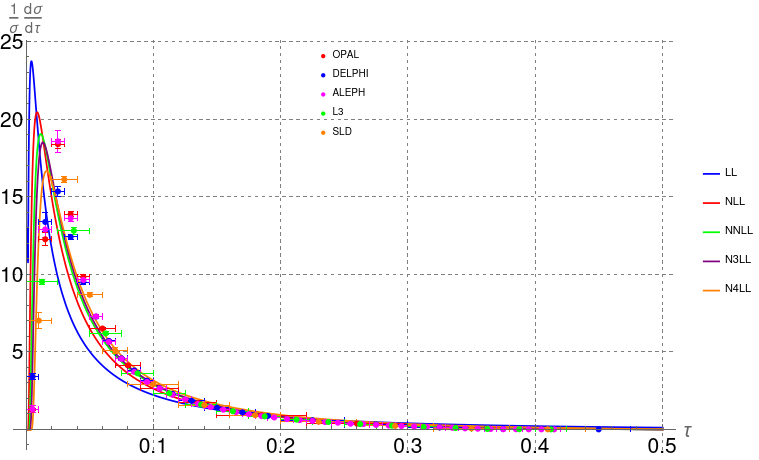
\includegraphics[width=\textwidth]{figures/Thrust_differential_distribution_with_xerr.png}
    \caption{Plot of \cref{eq:resummed_R} for different logarithmic accuracy orders, with coupling $\alpha_s(m_Z) = 0.118$.}
    \label{fig:Thrust distribution with data}
\end{figure}

\begin{figure}[htbp]
    \centering
    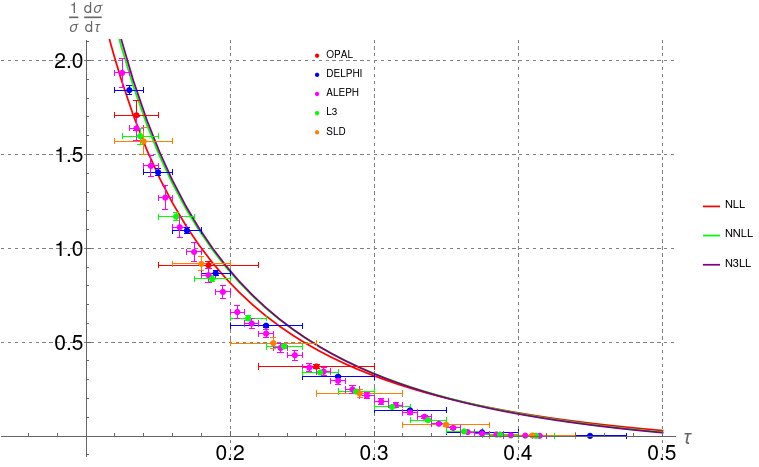
\includegraphics[width=\textwidth]{figures/Resummed_tail_region.png}
    \caption{Zoom-in in the tail region of the resummed thrust differential distribution \cref{eq:resummed_R} for different logarithmic accuracy orders, with fixed scale $\alpha_s = 0.118$.}
    \label{fig:resummed tail region}
\end{figure}

We also observe that the tail of the distribution (\Cref{fig:resummed tail region}) is not well described by the resummed expression, this is as expected since the resummation tackles the problem of large logarithms in the $\tau \to 0$ region,
for the tail of the distribution we would need to include the fixed order corrections. We'll see in the next section how to combine the resummed expression with the fixed order corrections to obtain a more accurate prediction
in a greater range of $\tau$.
\end{document}